\CHAPTER{The LIGO detector}
\label{chapter2}
%\doublespace

In this chapter I will explain how the LIGO detectors work.

\section{Arms, cavities, etc}

The purpose of the LIGO detectors is to measure the faint
oscillations of spacetime imparted by far-away astrophysical
processes.  Through clever design and careful engineering, these
machines are capable of resolving these tiny perturbations from the
much louder sea of noise on the surface of the Earth.

As we have seen, a passing gravitational wave modulates the optical
path length of light passing between inertial test
masses.  To exploit this effect and build a detector around it, we
need to arrange to have inertial test masses.  We need to be able to
tell the difference between phase perturbations due to the
gravitational wave and phase perturbations inflicted by our light
source.  We need to eliminate sources of phase variations that would
be louder than the effect we wish to measure.  

\begin{itemize}
\item We approximate inertial test masses by hanging the optics as
  pendula.  These act as inertial masses above the pendulum resonance.
\item We build a Michelson interferometer for its common-mode noise
  rejection.  This is nicely compatible with the tensor action of
  gravitational waves.
\item To enhance the effect from a passing gravitational wave, we make
  the arms as long as possible.  To further enhance the response, we
  have the light travel this path many times, by using resonant cavities.
\item To increase the optical response to a gravitational wave, we
  increase the light power in the interferometer by using power
  recycling.
\end{itemize}

\section{A single cavity}

Our first impulse might be to build a single resonant cavity to use as
a gravitational wave detector.  Consider the two-mirror system in
Figure~\ref{fig:fabry-perot}.  By suspending these two mirrors as
pendula, we can simulate intertial test masses.  The resonant optical
cavity is of ubiquitous utility in LIGO, so this discussion will be of
general interest.

Here we will ignore the spatial distribution of light, and its
polarization.  Despite these simplification, the results will have
wide applicability.

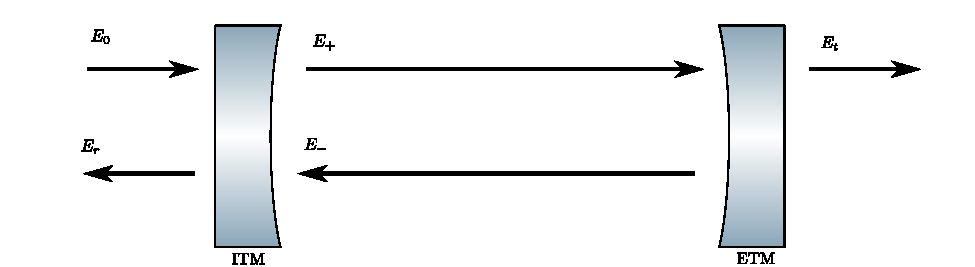
\includegraphics[]{figures/cavity.pdf}

Solving for the fields, we get the amplitude transmission and
reflection coefficients for the cavity:
%
\begin{align}
t_c := & \frac{E_t}{E_0} = 
         \frac{-t_1 t_2 \exp i\phi}
              {1 - r_1 r_2 \exp i2\phi} \\
r_c := & \frac{E_r}{E_0} = 
         \frac{r_1 - \left({r_1}^2 + {t_1}^2\right)r_2 \exp{i2\phi}}
              {1 - r_1 r_2 \exp i2\phi}
\label{eq:cavity-reflectivity}
\end{align}
%
where $\phi$ is the phase accumulated by the field as it travels from
the first mirror to the second mirror.  The phase depends on both the
laser wavelength and the distance between the mirrors:
$\phi=2\pi(2L/c)\nu$.  The quantity $fsr=c/(2L)$ is the \emph{free
  spectral range}.  It is often useful to write the cavity
reflectivity in the form of a rational transfer function (poles and
zeros):
%
\begin{equation}
r_c(s) = \mathop{\Huge{\Pi}}\limits_{n=-\infty}^{\infty} \frac {s-z_n} {s-p_n}
\end{equation}

For the arms of a gravitational wave detector, we set $r_2$ as close
to unity as possible.  We are interested in the phase of the reflected
field. 
 
Recall that the phase at frequency $\omega$ imparted by a pole at
frequency $\omega_0$ is $\tan^{-1}\left(-\omega/\omega_0\right)$; a
zero at the same frequency subtracts this same phase.  For a maximally
over-coupled cavity (i.e. with $r_2 = 1$), the cavity pole and cavity
zero are equal and opposite, so contribute equal phase ($\tan^{-1}$ is odd).

Changing the one-way phase of the arm by $\phi$ results in a phase 
change of
\begin{equation}
\phi_r = 2 \tan^{-1} \left( 2 f_{fsr} \frac{\phi}{\omega_0} \right)
\end{equation}
where $\omega_0$ is the cavity pole.  Taking the derivative, we find the \emph{phase gain}:
\begin{equation}
  \frac{d \phi_r}{d \phi} = 2 \left[1 + \left(\frac{2 f_{fsr} \phi}{\omega_0}\right)^2 \right]^{-1} \frac{2 f_{fsr}}{\omega_0}
\end{equation}
The phase gain on resonance is $2 f_{fsr} / \omega_0 \approx 140$. This phase gain decreases as we detune the cavity further from resonance, but it is not seriously diminished until the cavity detuning approaches the cavity pole.

\section{A Michelson}
\begin{figure}
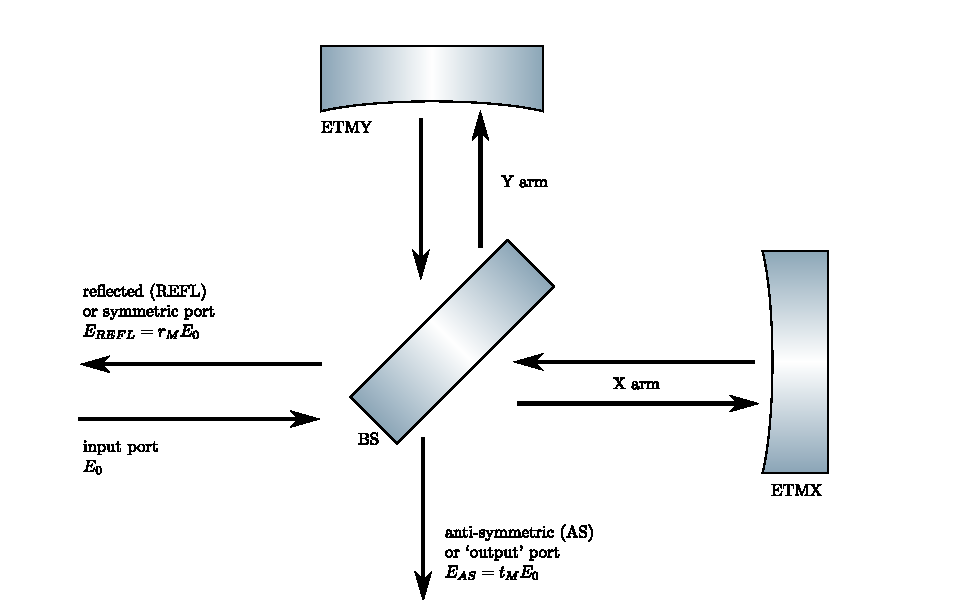
\includegraphics{figures/michelson.pdf}
\caption[Michelson interferometer]{\label{fig:michelson}Michelson interferometer}
\end{figure}

By a convenient coincidence, a Michelson interferometer is ideally
suited to gravitational wave detection.  A suitably polarized wave
directly excites the differential mode of the Michelson, while the
Michelson simultaneously provides huge level of common mode noise
rejection.

If we assume a perfect beamsplitter, the transmission and reflection
coefficients for the Michelson are:
%
\begin{align}
t_M  &= \frac{1}{2}\left(r_x \exp \{i2\phi_x\} - r_y \exp\{i2\phi_y\} \right) \\
r_M  &= \frac{1}{2}\left(r_x \exp \{i2\phi_x\} + r_y \exp\{i2\phi_y\} \right)
\end{align}
where $r_{\{x,y\}}$ are the amplitude reflectivities of the x- and y-arm mirrors, and $\phi_{\{x,y\}}$ are 
the phases accumulated as the light travels from the beamsplitter to end mirrors.  It is useful to change
our variables to express these quantities in terms of the differential and common reflectivies and phases.
Make the substitutions
%$\phi_- = \phi_x - \phi_y$ and 
%$\phi_+ = \phi_x + \phi_y$, i.e. 
$\phi_x = (1/2)\left(\phi_+ + \phi_-\right)$
$\phi_y = (1/2)\left(\phi_+ - \phi_-\right)$
%% which gives
%% \begin{align}
%% t_M  &= \frac{1}{2}\left(r_x e^{i2\phi_x} - r_y e^{i2\phi_y} \right) \\
%% r_M  &= \frac{1}{2}\left(r_x e^{i2\phi_x} + r_y e^{i2\phi_y} \right)
%% \end{align}
%%
%% \begin{align}
%% t_M  &= \frac{1}{2}\left(r_x e^{i\left(\phi_+ + \phi_- \right)} - r_y e^{i\left(\phi_+ - \phi_-\right)} \right) \\
%% r_M  &= \frac{1}{2}\left(r_x e^{i\left(\phi_+ + \phi_- \right)} + r_y e^{i\left(\phi_+ - \phi_-\right)} \right) 
%% \end{align}
%%
%% \begin{align}
%% t_M  &= \frac{1}{2} e^{i\phi_+} \left(r_x e^{i \phi_- } - r_y e^{-i \phi_-} \right) \\
%% r_M  &= \frac{1}{2} e^{i\phi_+} \left(r_x e^{i \phi_- } + r_y e^{-i \phi_-} \right) 
%% \end{align}
%%
%% Now we can also separate the arm reflectivity into common and differential reflectivity, using 
and $r_x = (1/2)(r_+ + r_-)$ and $r_y = (1/2)(r_+ - r_-)$:
%
\begin{align}
t_M  &= \frac{1}{2} e^{i\phi_+} \left( r_+ i \sin \phi_- + r_- \cos \phi_- \right)\\
r_M  &= \frac{1}{2} e^{i\phi_+} \left( r_+ i \cos \phi_- + r_- \sin \phi_- \right) 
\end{align}
%
Using $P_{AS} = P_{BS} \left|t_M\right|^2$ and $P_{REFL} = P_{BS}
\left|r_M\right|^2$ we can compute the power at the antisymmetric and
reflected ports:
%
\begin{align}
P_{AS}   &=  \frac{1}{4}P_{BS}\left( {r_+}^2 \sin^2 \phi_- + {r_-}^2 \cos^2 \phi_-\right) \\
P_{REFL} &=  \frac{1}{4}P_{BS}\left( {r_+}^2 \cos^2 \phi_- + {r_-}^2 \sin^2 \phi_-\right) 
\end{align}

The power transmitted through the Michelson at the dark fringe is the
\emph{contrast defect},
%
\begin{equation}
c_d = \frac{P_{AS}}{P_{BS}} = \frac{1}{4}\left(r_-\right)^2.
\end{equation}

\section{Michelson with Fabry-Perot arms}

To consider a Michelson interferometer with Fabry Perot cavities for
arms, we can substitute the cavity reflectivity into our Michelson
equations.

It is easier to simply put in the phase gain.

\section{Power recycling}

The Michelson interferometer tuned to a dark fringe for the laser
carrier sends most of the laser power back towards the laser.  Instead
of discarding this power, it can be sent back into the Faby-Perot
Michelson interferometer.  This is done by adding an additional
mirror, the \emph{power recycling mirror}, that forms a resonant
cavity with the rest of the interferometer.  Choosing the reflectivity
of the power recycling mirror to match the effective reflectivity of
the rest of the interferometer makes this cavity critically coupled;
ideally all of the laser carrier is coupled into the interferometer
and very little is reflected.  Most of the light stays in the
interferometer until it is lost to scattering or absorption.

\section{The coupled cavity pole}

We can consider the Fabry-Perot Michelson, or, really, any assembly of
mirrors as a single compound mirror with a complex-valued,
frequency-dependent reflectivity.  In particular, we can model the
power-recycled Fabry-Perot Michelson as a three mirror cavity.

The dynamics of three-mirror cavities are treated comprehensively in
chapter 4 of Malik's thesis~\cite{Rakhmanov2000Dynamics}.

To find the transfer function of the coupled cavity, we can simply
substitute the cavity reflectivity function $r_c(\phi)$ given in
equation~\ref{eq:cavity-reflectivity} into itself.  

To find the cavity pole of the combined cavity, a good approximation
results if we first compute the reflectivity of the shorter cavity on
resonance, and substitute this into the expression for the cavity pole.
We get:

\begin{equation}
f_{cc} \approx \frac{1}{2\pi} f_{fsr} \log \left(\frac{r_3 - r_1}{1 - r_1 r_3} r_2\right)
\end{equation}



\section{Interferometer Sensing and Control}

The laser light incident on the interferometer is phase-modulated at
several frequencies, producing optical sidebands on the laser carrier.
Light extracted from the interferometer at its various ports is
incident on photodiodes; the photodiode signals are demodulated to
produce signals.

\cite{Fritschel2001Readout}


%%%%%%%%%%%%%%%%%%%%%%%%%%%%%%%%%%%%%%%%%%%%%%

\section{Determination of LIGO cavity lengths and mirror reflectivities}

The lengths of cavities and reflectivities of mirrors in LIGO are
all driven by a small number of design decisions. This document is
intended to be a brief and friendly derivation of some of these values.
Definitive references are \cite{LigoFreqResponse97} or \cite{Fritschel2001Readout}.
A more general reference is \cite{S5InstrumentPaper}.

In this document I simply use the plane-wave approximation for fields
inside cavities. This introduces certain inaccuracies, as, for example,
I ignore gouy phase. Nonetheless, comparison to the actual dimenions
of LIGO shows good agreement. Furthermore, I present cavity equations
without any derivation. Derivations may be found in almost any LIGO
thesis or optics book. I have tried to use symbols relatively standard
within LIGO. My own derivations may be found in the appendix.

It is useful to draw a distinction between macroscopic and microscopic
lengths. Macroscopic lengths are those derived in this document and
used in detector engineering, with magnitudes ranging from kilometers
down to centimeters or millimeters. Microscopic lengths are those
on the order of the wavelength of light and smaller, sometimes \emph{much}
smaller. Microscopic lengths are never determined explicitly; instead
they are controlled by servo systems to hold cavities on resonance.
When we say that a cavity is a certain macroscopic length, we retain
the freedom to adjust the microscopic length to attain resonance.


\subsection*{Arm length}

How big a detector can you build? The physical length of the detector
sets the conversion from displacement to strain. Simply making the
detector longer will make any fixed displacement noises into smaller
strain noises-so we want the detector as large as possible. How big
you can build is usually a result of geography, money, and politics.
LIGO got

\[
\boxed{{L_{+}=4000\text{{\ meters}}}}
\]


The cavity length determines the free-spectral-range:

\[
f_{fsr}\equiv\frac{c}{2L_{+}}\approx37.5\text{ kHz}
\]



\subsection*{Bandwidth}

In the absense of a signal extraction mirror, there is a trade-off
between the detector's sensitivity and its bandwidth. As the storage
time in the arm becomes longer and longer (either by making the arm
longer, or by increasing its finesse), the sensitivity to gravitational
waves increases commensurately. However, sensitivity to waves whose
period is shorter than the storage time of the arm is attenuated.
Thus there is a trade-off between sensitivity and bandwidth. The first
order of business is to choose the bandwidth. LIGO chooses:

\[
f_{c}=90\text{\ Hz}
\]
Together, the free spectral range and the arm cavity pole determine
the cavity finesse:

\[
\mathcal{F}=\frac{f_{FSR}}{2f_{c}}\approx210
\]



\subsection*{Test mass reflectivities}

Knowing our desired finesse allows us to choose the mirror reflectivities.
The finesse is uniquely determined by the fraction of circulating
power that remains in the cavity after each roundtrip, which is given
by a product of the mirror reflectivities and $r_{L}=\sqrt{1-L}$
where L represents losses due to scattering, absorption, etc. 
\[
\mathcal{F}\approx-\frac{\pi}{\log r_{1}r_{2}r_{L}}
\]


This relation fixes the product $r_{1}r_{2}$, leaving the ratio $r_{1}/r_{2}$
as a free parameter. This ratio determines the coupling of the cavity,
from maximally over-coupled ($r_{2}\rightarrow1$), to critically
coupled ($r_{1}=r_{2}$), or to cavity at all ($r_{1}\rightarrow1$).
How do we choose the coupling? Intuitively, we want to couple as much
light as possible into the cavity. In one point of view, this is so
there is as much light as possible present inside the cavity to be
phase modulated by the gravitational wave. The power gain inside the
cavity is given by
\[
g^{2}=\frac{1-r_{1}{}^{2}}{\left(1-r_{1}r_{2}\right)^{2}}
\]
To maximize this, we want $r_{1}$ as small as possible, so we make
the ETM as reflective as possible. It turns out that maximal over-coupling
is the way to go. The best super-polished mirrors we can buy have
transmissivities of 10 ppm, which gives

\[
r_{2}=\sqrt{{1-10\times10^{-6}}}\approx0.999995
\]
Solving equation 1, we find:
\[
r_{1}\approx0.985
\]
\textcolor{blue}{{[}I also need to put in a discussion of losses.
The cavity losses are not negligible. The Optickle model gives losses
of 70ppm for each HR surface, which far exceeds the ETM transmission.
Then I can derive a reasonable value of rc, the cavity reflectivity
on resonance, which sets the RM reflectivity.{]}}


\subsection*{Power Recycling - Recycling Mirror}

With the FP Michelson interferometer tuned to the dark fringe, all
of the light not lost in the arm cavities is reflected back towards
the laser source. To send this light back into the interferometer,
we add a power recycling mirror, which forms a resonant cavity with
the FP Michelson. We choose the reflectivity of the recycling mirror
to make the cavity critically-coupled for the carrier. 

With the Michelson on a dark fringe, the Michelson reflectivity is
given by the cavity reflectivity on resonance:

\[
r_{c}=\frac{r_{1}-r_{2}}{1-r_{1}r_{2}}
\]
\textcolor{blue}{{[}Need to add losses to that expression in order
for this to work out.{]} }We choose:

\[
r_{RM}{}^{2}=0.97
\]


\emph{The recycling mirror transmission is chosen to match the losses
of the rest of the system.}


\subsection*{Length degrees of freedom}

\textcolor{blue}{I should explain that we transform lx, ly, Lx, and
Ly into l- (Michelson asymmetry), l+ (PRC length), L+ (CARM length),
and L- (DARM length) degrees of freedom. I should show that the PRC
{}``sees'' the average distance of the Michelson arms (l-), etc.}


\subsection*{Power Recycling - PRC cavity length}

We need to have some radio-frequency sidebands in order to implement
the heterodyne scheme that is used to control most of the interferometer.
Its frequency is chosen to be several tens of MHz, and to be approximately%
\footnote{If the sideband were perfectly anti-resonant in the arms, then the
first harmonic would be resonant, which is undesirable.%
} anti-resonant in the arm cavities. We choose:

\[
f_{RF}\approx24.5\mathrm{{\ MHz}}
\]


The RF sidebands must fit in the power recycling cavity. The resonant
conditions for the carrier and for the sideband in the PRC are slightly
different. Because the carrier is resonant in the (strongly over-coupled)
arm cavities, it sees a sign flip in reflection from the arms that
is not seen by the sideband. The carrier is actually \emph{anti-}resonant
in the PRC until the arms come into resonance and this extra sign
flip comes into play. The minimum length of the PRC that satisfies
this requirement occurs when the carrier accumulates $\pi$ radians
more phase than the lower sideband over a round-trip traversal of
the cavity. (The upper sideband, in turn, acquires $\pi$ radians
more than the carrier, putting it $2\pi$ above the lower sideband,
making them simultaneously resonant. The carrier gets its final $\pi$
radians on reflection from the over-coupled arm.) Instead of relying
on intuitive arguments, we can write down equations for the conditions
of resonance:

\begin{eqnarray}
\exp \left\{i (2l/c)\omega_{0}  \right\} &=& -1 \\
\exp \left\{i (2l/c)(\omega_{0} \pm \omega_{rf}) \right\} &=& +1
\end{eqnarray}Solving these%
\footnote{Remember the multivaluedness of the logarithm, i.e. $\log1=i2\pi n$
for all integers $n$.%
}, we find a nice relationship between the cavity length and the RF
wavelength $\lambda_{rf}=c/f_{rf}\approx12\text{ meters}$:

\[
2l_{+}=\lambda_{rf}\left(m+\frac{1}{2}\right)
\]
where m is any integer. The length corresponding to $m=0$ is inconveniently
short%
\footnote{I assume this is the reason...%
}, so we choose $m=1$, giving a power recycling cavity length of:

\[
\boxed{{l_{+}=9.18\text{{\ meters}}}}
\]


\emph{The PRC length is set to allow simultaneous resonance of the
carrier and sidebands in the power recycling cavity.}


\subsection*{Schnupp asymmetry}

Now that we have the RF sidebands resonant in the recycling cavity,
we need to get them to the output port. 

A Michelson with identical arms has no frequency selectivity; in principle
even white light would experience bright and dark fringes. Introducing
an offset breaks this degeneracy, as the offset allows higher frequency
waves to accumulate more phase than slower frequencies. Introducing
a macroscopic difference in the arm lengths separates the carrier
fringes from the sideband fringes. In the longer arm, now, the lower
sideband accumulates less phase than the carrier, and the upper sideband
accumulates a bit more. When the beams from the two arms recombine,
the phase difference now depends on the frequency. With such an asymmetry,
the Michelson can be simultaneously reflective of the carrier and
partially transmissive of the sidebands. 

How much sideband transmission do we need? The Michelson is acting
as the second mirror in a resonant cavity. If we want to have perfect
transmission of the sideband to the output port, then the power recycling
cavity must be critically coupled for the sideband. This occurs when
the Michelson transmission of the sideband is equal to the transmissivity
of the RM.

This scheme for getting the sideband to the {}``dark'' port is attributed
to Lisa Schnupp, and the offset is called the Schnupp asymmetry.

The Michelson reflectivity for the sideband is:

\[
r_{M}=\cos\frac{2\pi f_{rf}l_{-}}{c}
\]


\textcolor{blue}{{[}The fringe of the lower sideband lags that of
the carrier, and the upper sideband leads the carrier. But because
the carrier itself is on a dark fringe, the transmission of both the
upper and lower sidebands turns out to be the same.{]}}

Solving $r_{M}{}^{2}=0.97$ in order to match the RM, we find a Schnupp
asymmetry of

\[
l_{-}=34\text{\ cm}
\]
\textcolor{blue}{{[}The actual situation is more complicated. Sigg
explains, in \href{http://www.ligo.caltech.edu/docs/T/T030066-00.pdf}{T030066},
April 2003:}
\begin{quote}
\textcolor{blue}{The Schnupp asymmetry of the two 4K interferometer
is too short by 55 mm. The design required the reflected rf sideband
amplitude to be +10\% (under-coupled). The current setup indicates
an amplitude of \textendash{}7\% (over-coupled) when the system is
fully heated. This results in a sign change of the reflected signal
used to control the laser frequency during locking or while the thermal
heating takes effect. Worse, the signal is likely to become useless
when the rf sideband amplitude goes through zero. It looks like the
Schnupp asymmetry has been calculated correctly for the 2K interferometer
and later applied to the 4K interferometers without taking into consideration
the difference in modulation frequency. }
\end{quote}
\textcolor{blue}{M.Evans write-up in \href{http://www.ligo.caltech.edu/docs/T/T030089-00.pdf}{T030089},
{}``Non-Resonant Sidebands and the 4k Schnupp Asymmetry'' also looks
useful.{]}}

\emph{The Schnupp asymmetry sets the coupling of the sideband to the
antisymmetric port.}


